\documentclass[tikz,border=3.14mm]{standalone}
\begin{document}
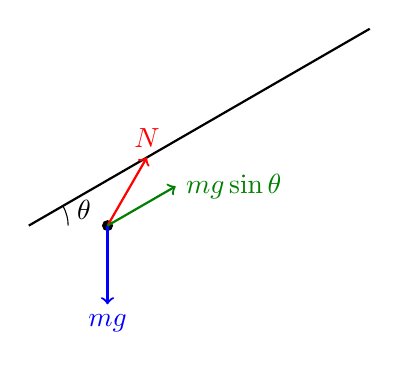
\begin{tikzpicture}
    % Define the angle of inclination
    \pgfmathsetmacro{\angle}{30}
    
    % Draw the inclined plane
    \draw[thick] (0,0) -- (\angle:5);
    
    % Draw the object
    \fill (1,0) coordinate (a) circle (2pt);
    
    % Draw and label the forces
    \draw[->,thick,red] (a) -- ++(90-\angle:1) node[above] {$N$};  % Normal force
    \draw[->,thick,blue] (a) -- ++(-90:1) node[below] {$mg$};  % Gravitational force
    \draw[->,thick,green!50!black] (a) -- ++(\angle:1) node[right] {$mg\sin\theta$};  % Component of the gravity along the incline
    
    % Label the angle
    \draw (0.5,0) arc (0:\angle:0.5);
    \node at (0.7,0.2) {$\theta$};
\end{tikzpicture}
\end{document}